% Chapter Template

\chapter{Software Architecture} % Main chapter title

\label{ChapterX} % Change X to a consecutive number; for referencing this chapter elsewhere, use \ref{ChapterX}

\lhead{\emph{Software Architecture}} % Change X to a consecutive number; this is for the header on each page - perhaps a shortened title

%----------------------------------------------------------------------------------------
%	SECTION 1
%----------------------------------------------------------------------------------------

\section{Version}

\begin{tabular}{| p{1.5cm} | p{2cm} | p{9cm} | p{1.5cm} |}
	\hline
	Version & Date 		& Change & Author \\ \hline
	0.1 	& 8.10.2014 		& Setup document  										& JR \\ \hline
	0.2 	& 12.10.2014		& Class diagrams										& JR \\ \hline
	0.3 	& 16.10.2014		& Text													& JR \\ \hline
	0.4 	& 20.10.2014		& Activity diagram										& JR \\ \hline
	1.0 	& 21.10.2014		& Grammar, Diagram fixes								& JR \\ \hline
	1.1 	& 22.10.2014		& Adding description of all business logic classes, approach and extended introduction & JR \\ \hline
	1.2 	& 23.10.2014		& Grammar & JR,LR \\ \hline

\end{tabular}

\section{Introduction}

This document describes the software architecture of the context extraction test framework. 
The context extraction test framework will perform automated text extraction on a set of HTML test data with two to three different text extraction algorithms. After measuring the performance of each algorithm, an output file with the measured results is generated.

\section{Logical view}

\subsection{Approach}
This section describes the approach for elaborating the software architecture. 
The following figure from the software requirement specification is the basis for elaborating the software architecture.

%\begin{landscape}

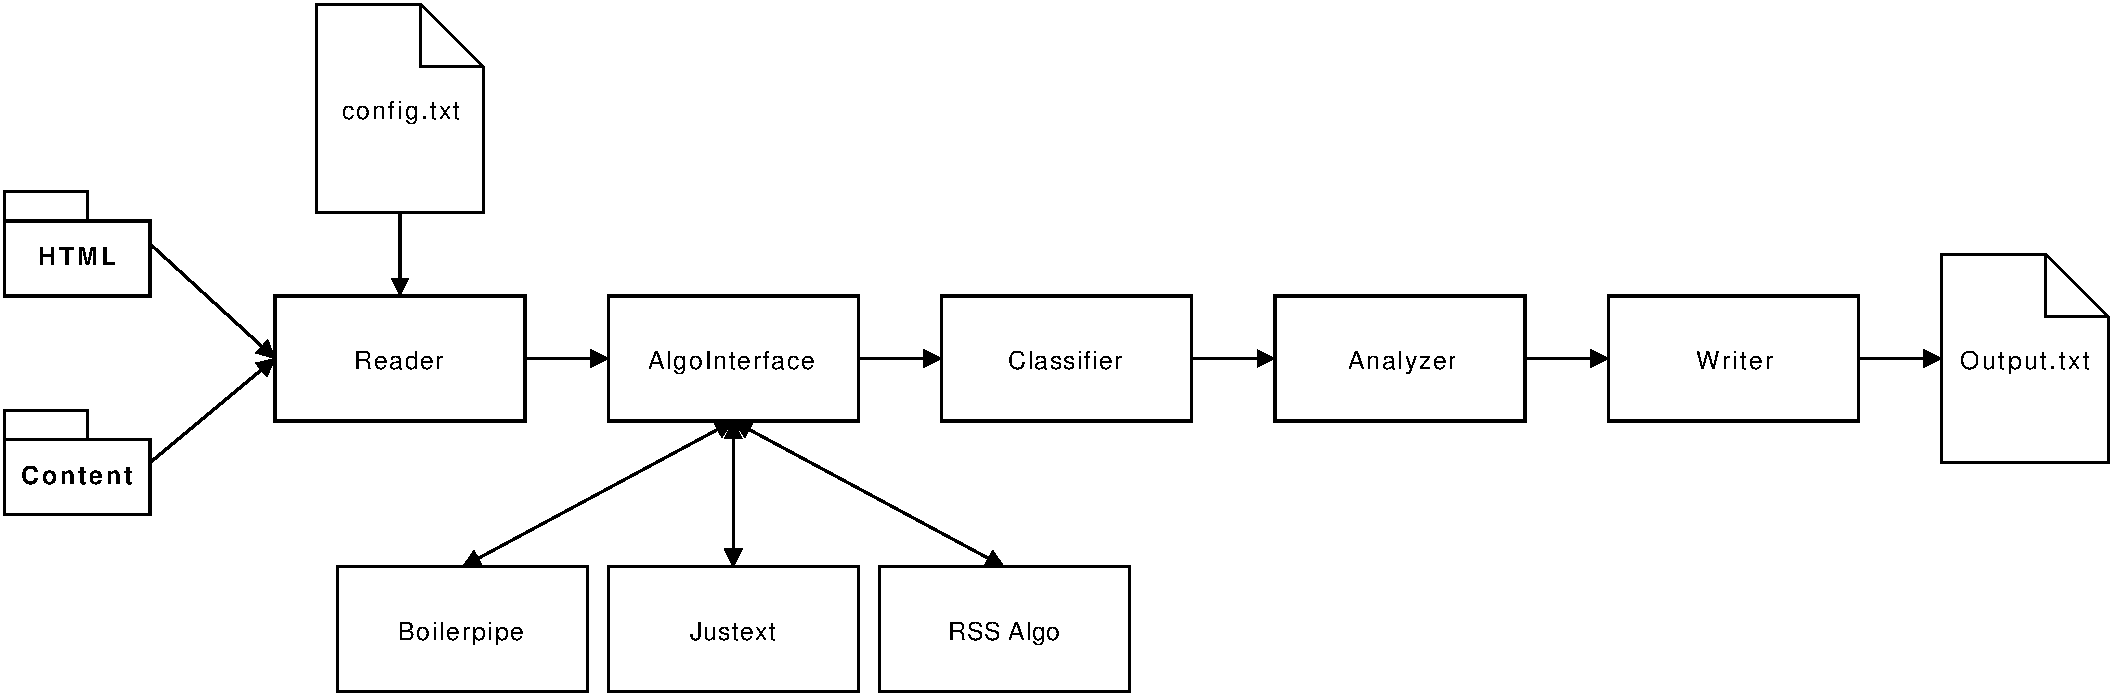
\includegraphics[width=15cm]{Figures/App_overview.pdf}

%\end{landscape}

First all possible entities in the domain are identified and a data model is elaborated. The data model is described in \ref{subsec:Data model}. Then the business logic is researched based on the figure above. With this knowledge, the five packages main, reader, classifier, analyzer and writer are defined. The functions for each package is then evaluated and split into single classes. During the implementation of the first approach, some classes are adapted due to unforeseen circumstances. The outcome is described in \ref{subsec:Business Logic}.
\pagebreak

\section{Data model}
\label{subsec:Data model}

The following diagram shows the data model of the application. 

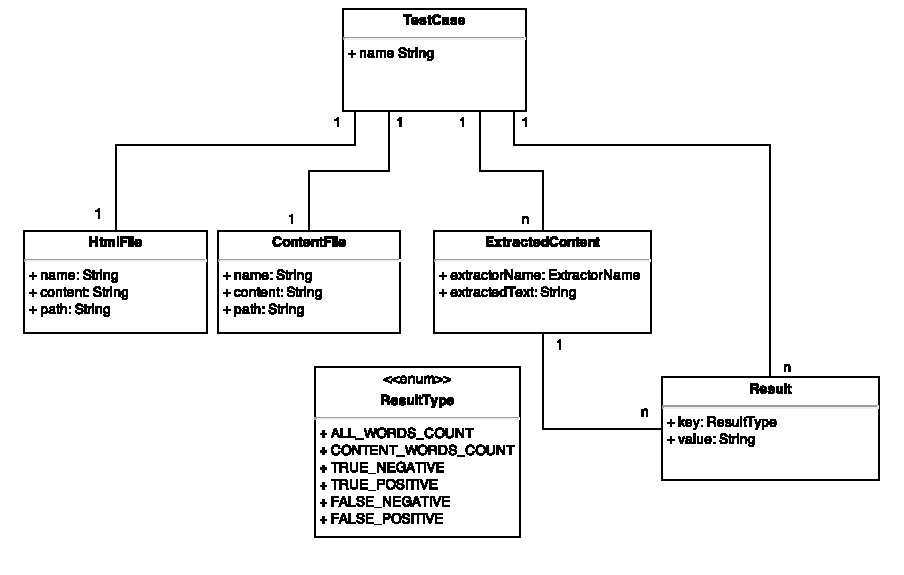
\includegraphics[width=14cm]{Figures/dataModel.pdf}


\subsection{TestCase}
A TestCase object is generated for each HTML/content file pair in the input folders. A TestCase has a a name which is unique and which matches the name of the content and HTML file.

\subsection{HtmlFile}
Each TestCase has an HtmlFile object. It contains the content of the actual HTML file as String and the file path.

\subsection{ContentFile}
Each TestCase has a ContentFile object. It contains the content of the actual text file as String and the file path.

\subsection{ExctractedContent}
Each TestCase can have multiple ExctractedContent objects. Each of them represents a result of a content extraction from an extractor such as Justext or Boilerpipe.

\subsection{Result}
A TestCase or an ExctractedContent object can have Result objects. The results are key value pairs which represent analytical data. An example for a Result related to a TestCase would be the word count of the content file, which is generally valid. An example for a Result related to an ExctractedContent would be the word count of true negative words, which is only valid for one specific ExctractedContent.


\begin{landscape}

\section{Business Logic}
\label{subsec:Business Logic}

The following diagram shows the business logic of the application. The diagram does not show all of the classes but the most important ones. 

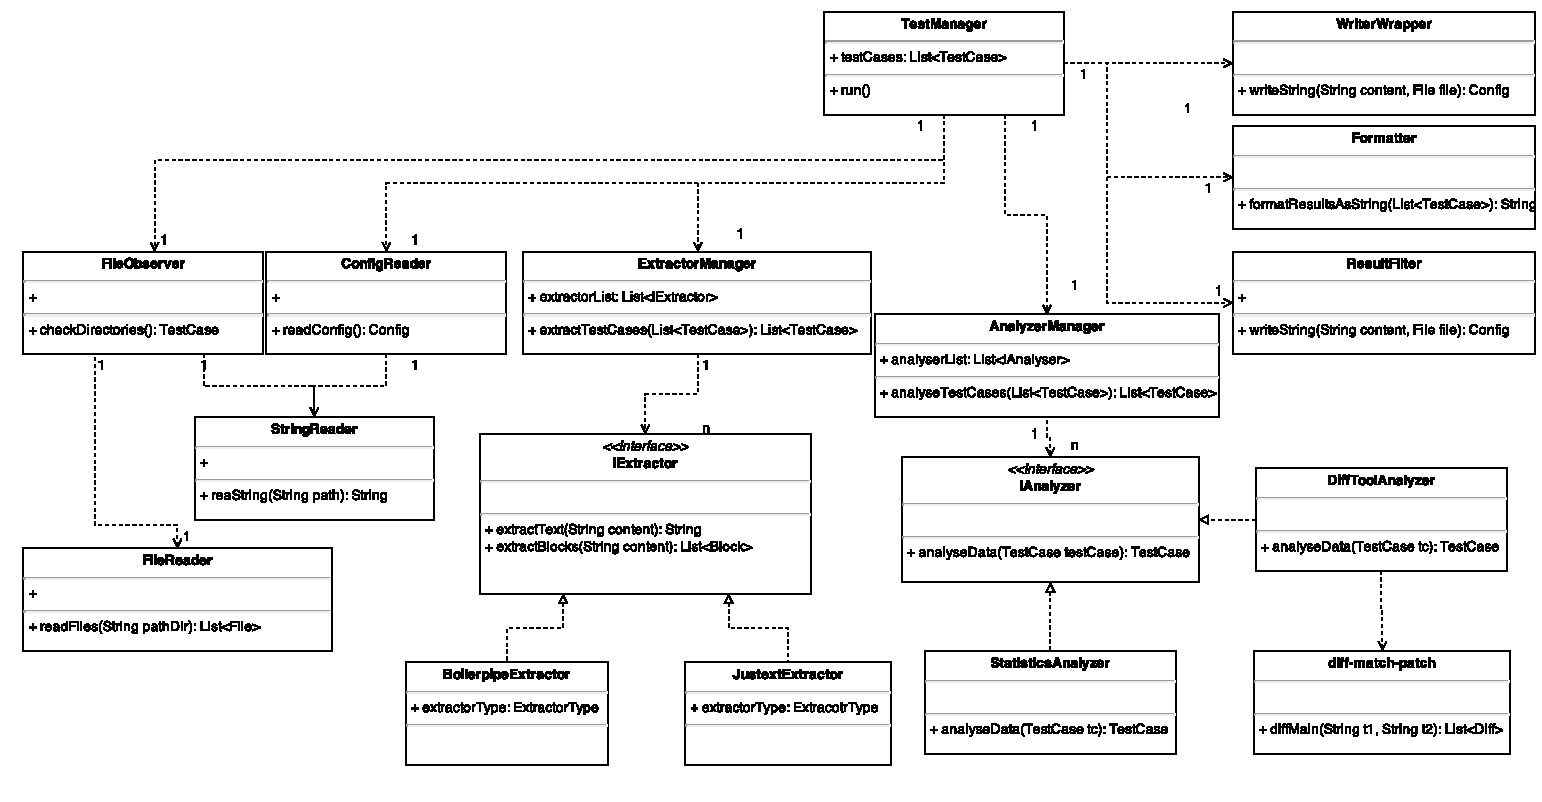
\includegraphics[width=23cm]{Figures/architecutre.pdf}

\end{landscape}

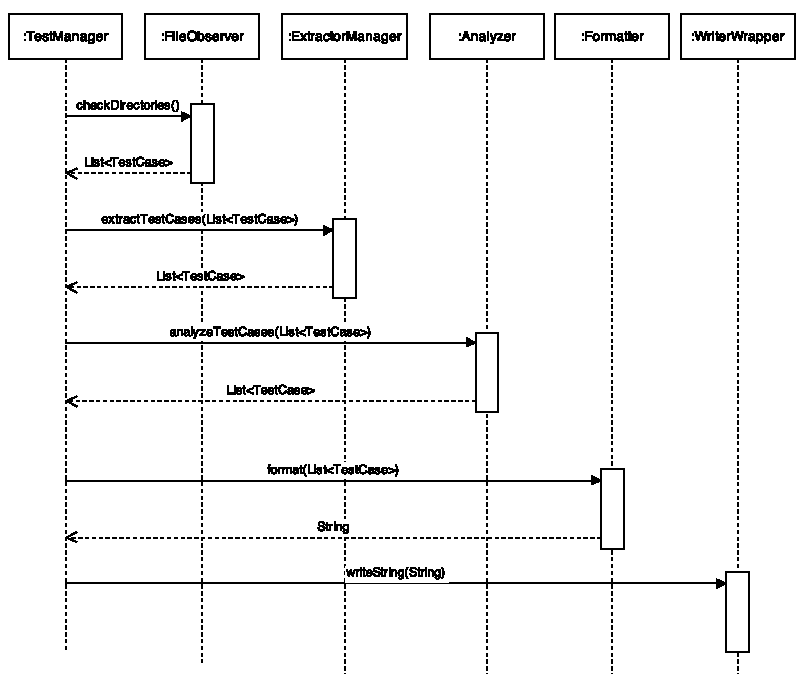
\includegraphics[width=15cm]{Figures/activityDiagram.pdf}

The data model is passed through the business logic and is enriched with data during the test procedure. First the input directories are checked for files by the FileObserver and TestCases are generated for each file pair with the same name. Then all the TestCases are then handed over to the ExtractorManager. The ExtractorManager extracts each TestCase with all available implementations of IExtractor and puts the Results into ExtractionResults. After that, all the TestCases are handed over to the Analyzer which runs each implementation of IAnalyzer. Each IAnalyzer produces at least one Result and puts it into the TestCase. To simplify the diagram, only two Analyzers are drawn. After generating some Results, the Formatter serializes the Result Objects into a String as a CSV table and the WriterWrapper persists the CSV data into an output file.

\pagebreak
\subsection{Description of single classes}

\begin{longtable}{p{4cm}|p{2cm}|p{8cm}}
\hline
\textbf{Class} &
\textbf{Package} &
\textbf{Description}
 \\ \hline
TestManager &
testManager &
The TestManager class manages the whole business logic that manages TestCase objects through the whole test process from reading the file content to writing the test results into an output file.
 \\ \hline
FileObserver &
reader &
The FileObserver class checks the HTML and content directory for files of the same name and creates TestCases from each found pair. The folders are checked with the FileReader class and the content of the files are read with the StringReader class.
\\ \hline
StringReader &
reader &
The StringReader class reads a text file and returns the content as String. The class is made for easier mocking of the BufferedReader so that testing of other classes which are dependent on external files becomes much easier.
\\ \hline
FileReader &
reader &
The FileReader class returns a File objects for each found file in a directory given by a parameter.
\\ \hline
ExtractorManager &
classifier &
The ExtractorManager manages all available Extractors. Each extractor which is used for the actual test must be initialized in this class and added to the ExtractorList. Each TestCase is then extracted by every IExtractor in the ExtractorList.
\\ \hline
IExtractor &
classifier &
The IExtractor is the interface to the different extractor. The interface is very lightweight. The parameter is the text that should be extracted and the return value is the extracted text.
\\ \hline
BoilerpipeExtractor &
classifier &
The BoilerpipeExtractor implements the IExtractor and is the interface to the Boilerpipe package. It handles all dependencies on the Boilerpipe package and returns the extracted content as a string.
\\ \hline
JustextExtractor &
classifier &
The BoilerpipeExtractor implements the IExtractor and is the interface to the Justext python program. The Java ProcessBuilder is used to create operating processes. One can then perform operating system commands and run the python script. The python script creates a text file with the extracted content which is read by the JustextExtractor class and returned as String.
\\ \hline
AnalyzerManager &          
analyzer &          
The AnalyzerManager manages all available analyzers. Each analyzer which is used for the actual test must be initialized in this class and added to the AnalyzerList. Each TestCase is then analyzed by every IAnalyzer in the AnalyzerList.
\\ \hline
IAnalyzer &
analyzer &
The IAnalyzer interface is a simple interface to the different analyzers. Each analyzer can generate one or more Result objects.
\\ \hline
WordCounterAnalyzer &
analyzer &
The WordCounterAnalyzer is a simple analyzer which counts all words of the content file, the HTML file and each extracted content.
\\ \hline
MatchingWordAnalyzer &
analyzer &
The MatchingWordAnalyzer compares the content file with each extracted content and calculates the values for true positive, true negative, false positive and false negative.
\\ \hline
Formatter &           
writer &           
The Formatter class formats a string from all TestCase objects as a CSV file structure. This means that a table with the Result keys as table header for each column is created. For each TestCase a row with the Result value field as values is added to the table. The outcome is a CSV file which can easily be imported into another program such as Excel so that one can work with the data.
\\ \hline
WriterWrapper &
writer &
The writer wrapper writes a string into a text file. It is used to wrap the BufferedWriter so that mocking and testing of dependent classes is easier.
\\ \hline
ConfigReader &
reader &
The ConfigReader class reads the config.txt file and puts the key value pairs into a HashMap.
\\ \hline
\end{longtable}


\section{Development view}

This chapter describes the used frameworks and tools which are used during the development process.

\subsubsections{Development tools}
\subsubsection{git}
\subsubsection{Gradle}
\subssubsection{Travic CI}
\subsubsection{Eclipse}
\subsection{Frameworks and APIs}

\subsubsection{Justext}

\subsubsection{Boilerpipe}

\subsubsection{TestNG}





\section{Process view}

\section{Physical view}